%% Adaptado a partir de :
%%    abtex2-modelo-trabalho-academico.tex, v-1.9.2 laurocesar
%% para ser um modelo para os trabalhos no IFSP-SPO

\documentclass[
    % -- opções da classe memoir --
    12pt,               % tamanho da fonte
    openright,          % capítulos começam em pág ímpar (insere página vazia caso preciso)
    %twoside,            % para impressão em verso e anverso. Oposto a oneside
    oneside,
    a4paper,            % tamanho do papel. 
    % -- opções da classe abntex2 --schwinn
    % Opções que não devem ser utilizadas na versão final do documento
    %draft,              % para compilar mais rápido, remover na versão final
    % paginasA3,  % indica que vai utilizar paginas em A3 
    % MODELO,             % indica que é um documento modelo então precisa dos geradores de texto
    % TODO,               % indica que deve apresentar lista de pendencias 
    % -- opções do pacote babel --
    english,            % idioma adicional para hifenização
    brazil              % o último idioma é o principal do documento
    ]{ifsp-spo-inf-ctds} % ajustar de acordo com o modelo desejado para o curso

% ---
% Pacotes importados para a utilização de referências
% ---

% ---
% Informações de dados para CAPA e FOLHA DE ROSTO
% ---
\titulo{PROVA DE CONCEITO - PROJETO TURMA DE ELITE}

% Trabalho individual
%\autor{AUTOR DO TRABALHO}

% Trabalho em Equipe
% ver também https://github.com/abntex/abntex2/wiki/FAQ#como-adicionar-mais-de-um-autor-ao-meu-projeto
\renewcommand{\imprimirautor}{
\begin{tabular}{lr}
     André Monteiro GOMES & SP3024059 \\
     Bianca Kaori HNG & SP3022455\\
     Luiz Henrique de Almeida e ALBUQUERQUE & SP3030199\\
     Natan da Fonseca LISBOA & SP3024784\\
     Patrícia Santos PASCHOAL & SP3022218
\end{tabular}
}


\disciplina{PI1A5 - Projeto Integrado I}

\preambulo{Trabalho apresentado ao Instituto Federal de Educação, Ciência e Tecnologia de São Paulo - Câmpus São Paulo - como parte dos requisitos para aprovação na disciplina Projeto Integrado I (PI1A5), do curso superior de Tecnologia em Análise e Desenvolvimento de Sistemas.}

\data{2021}

% Definir o que for necessário e comentar o que não for necessário
% Utilizar o Nome Completo, abntex tem orientador e coorientador
% então vão ser utilizados na definição de professor
\renewcommand{\orientadorname}{Professor:}
\orientador{DANIEL MARQUES GOMES DE MORAIS}


% ---


% informações do PDF
\makeatletter
\hypersetup{
        %pagebackref=true,
        pdftitle={\@title}, 
        pdfauthor={\@author},
        pdfsubject={\imprimirpreambulo},
        pdfcreator={LaTeX with abnTeX2 using IFSP model},
        pdfkeywords={abnt}{latex}{abntex}{abntex2}{IFSP}{\ifspprefixo}{trabalho acadêmico}, 
        colorlinks=true,            % false: boxed links; true: colored links
        linkcolor=blue,             % color of internal links
        citecolor=blue,             % color of links to bibliography
        filecolor=magenta,              % color of file links
        urlcolor=blue,
        bookmarksdepth=4
}
\makeatother
% --- 

% ----
% Início do documento
% ----
\begin{document}

\pretextual

\imprimircapa

\pdfbookmark[0]{\listfigurename}{lof}
\listoffigures*
\cleardoublepage

\pdfbookmark[0]{\contentsname}{toc}
\tableofcontents*

\textual

\chapter[Introdução]{Introdução}
A prova de conceito da aplicação será composta pelo cadastro e acesso da aplicação por um Administrador. Este processo, conforme demonstra a Figura 1, consiste em: criar o usuário administrador, fornecendo e-mail e nome, utilizando um usuário administrador previamente criado, acessar o link que foi enviado para o e-mail, fornecer senha e confirmação de senha. E assim que clicar no botão, além de criar o acesso, estará dentro da plataforma.

\begin{figure}[htb]
    \centering
	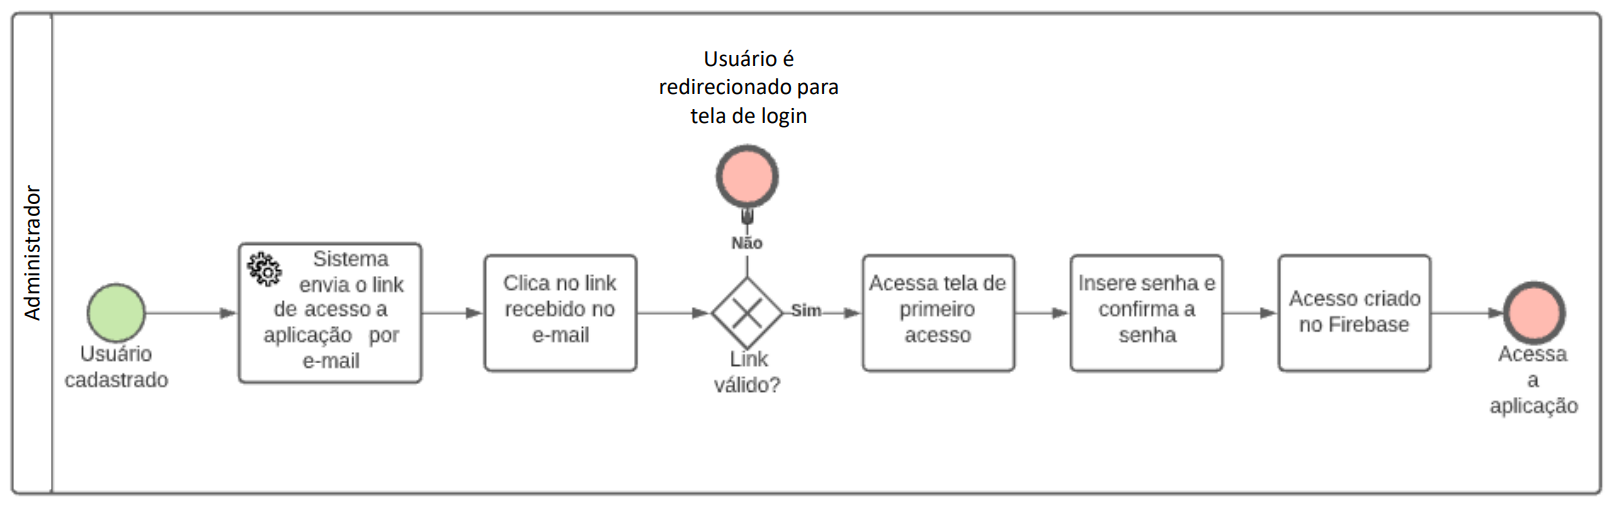
\includegraphics[width=16cm]{imagens/PrimeiroAcesso.png}
	\caption{Processo de Primeiro Acesso}
	\fonte{Os autores}
\end{figure}
\FloatBarrier

Caso o administrador já tenha sido cadastrado no sistema, basta realizar o processo de login na aplicação, conforme demonstrado na Figura 2.

\begin{figure}[htb]
    \centering
	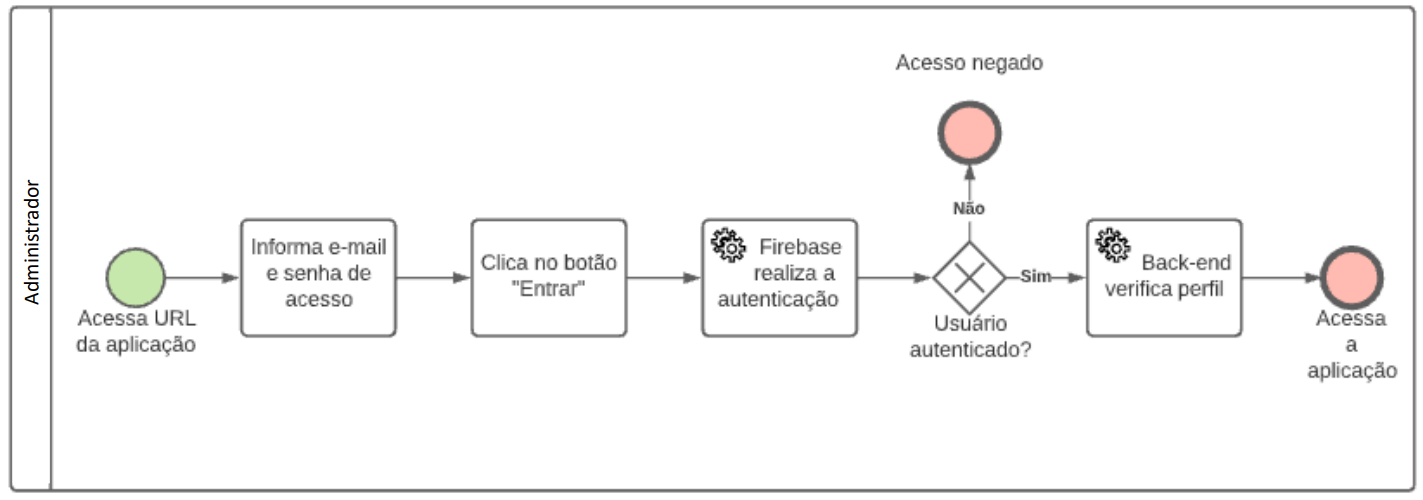
\includegraphics[width=16cm]{imagens/Login.png}
	\caption{Processo de Login}
	\fonte{Os autores}
\end{figure}
\FloatBarrier


Para que este processo possa ser concluído, todas as peças da arquitetura, conforme mostra a Figura 3, devem estar operando corretamente. A fim de simplificação, será considerado que pelo menos um usuário já foi cadastrado (o processo de cadastro do primeiro usuário é manual, realizando de forma direta a gravação da tupla no banco de dados e criação da URL de primeiro acesso). O início deste processo é através da interface web do projeto, escrita utilizando Angular 12 e servida através do Firebase Hosting.

\begin{figure}[htb]
    \centering
	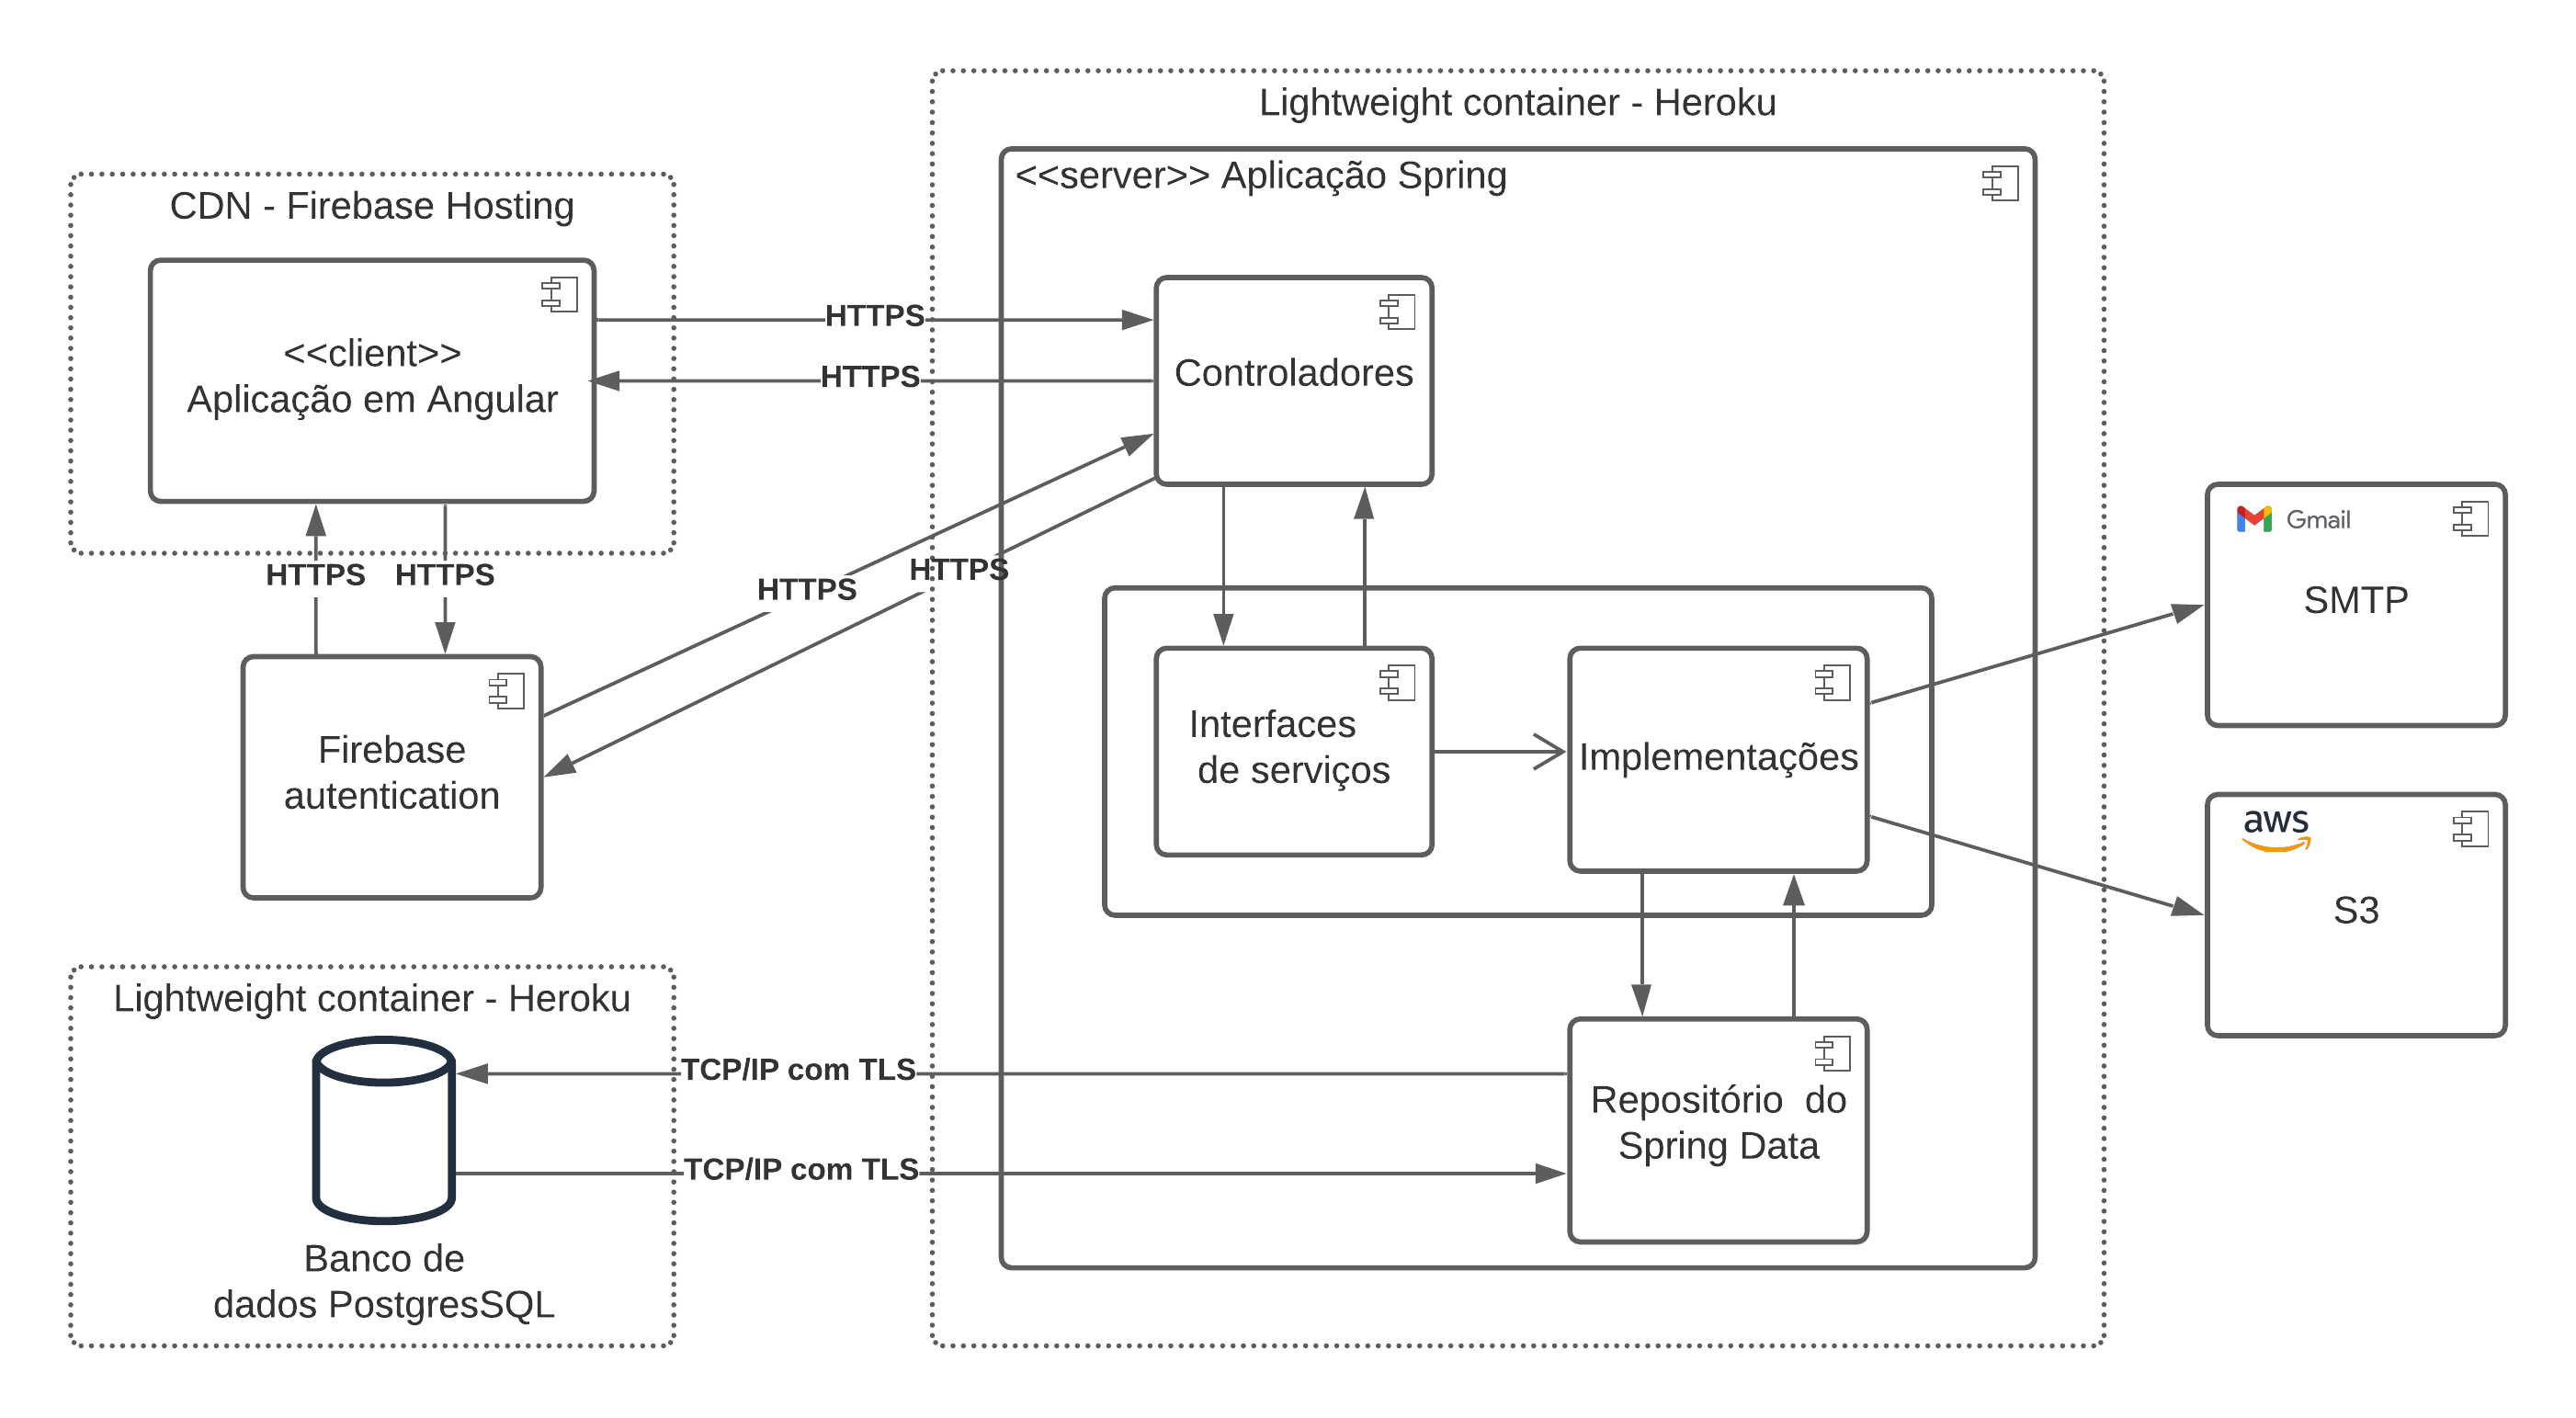
\includegraphics[width=16cm]{imagens/Arquitetura.png}
	\caption{Arquitetura da solução}
	\fonte{Os autores}
\end{figure}
\FloatBarrier

O projeto Angular foi criado utilizando a sua CLI (Command Line Interface) e o deploy no Firebase Hosting configurado utilizando a CLI do Firebase e realizada pelo Travis CI. Além disso, toda a interface foi construída utilizando o Angular Material Components, uma biblioteca de componentes que implementa o Design System Material Design, promovendo uma consistência de interface.

No momento que o usuário acessar a URL de login da aplicação, ele vai inserir o seu usuário e senha e realizar o login. O login da aplicação consiste em uma autenticação no lado cliente utilizando o @angular/fire, no qual a senha e e-mail são enviados para os servidores do Firebase. O cliente recebe de volta tokens que o identificam, e um destes tokens são utilizados para acessar endpoints protegidos do back-end.

O back-end é uma aplicação Java, escrita utilizando o framework Spring com as bibliotecas do ecossistema, hospedado em um dyno do Heroku. Este back-end também utiliza o MySQL para armazenar os dados pertinentes a aplicação, que está hospedado em um VPS da Oracle Cloud. Ele também utiliza a biblioteca de API de administração do Firebase (SDK Admin), que é utilizada tanto para autenticar usuários (verificando os tokens gerados para o cliente) quanto para criar os usuários (para que eles possam recuperar estes tokens no cliente).

Assim que o cliente concluir a autenticação do seu lado, ele realiza uma chamada ao back-end para verificar o papel do usuário e encaminhar para a interface adequada ao seu papel. Ao acessar a funcionalidade de criação do Administrador e criar o administrador, a requisição é enviada ao back-end, que realiza a requisição do envio de um e-mail com as informações de primeiro acesso. O envio de e-mail é realizado utilizando o servidor SMTP do Google, que é acessado utilizando as credenciais de um Gmail e Spring Email.

Quando o e-mail é recebido, o usuário que foi cadastrado, pode acessar o link, informar uma senha e então, um usuário será criado no Firebase Authentication, permitindo que este usuário possa acessar a plataforma

\chapter[Decisões Tomadas]{Decisões Tomadas}
Para a escolha do front-end, back-end, banco de dados, Firebase Authentication e envio de e-mails, levaram-se em consideração alguns critérios.

\section{Front-end}
Sendo uma aplicação de acesso restrito, consequentemente não necessitando de SEO, soluções de desenvolvimento SPA poderiam ser utilizadas no projeto com maior facilidade. Logo, o framework Angular foi escolhido. Ele provê uma forma de escrever aplicações em que o projeto pode escalar de tamanho sem perder produtividade no desenvolvimento. Também possui ecossistema, que vai desde o linting até a biblioteca de componentes, totalmente integrados e, com exceção da biblioteca de componentes, possui mínima dependência de bibliotecas externas ao framework.

\section{Back-end}
Para o back-end, a solução escolhida não necessitaria apresentar características específicas, como quantidade massiva de acessos simultâneos, alta concorrência, entre outros, a escolha foi pautada na experiência dos integrantes do grupo. Como a linguagem orientada a objetos que todos os integrantes do grupo já tinham estudado era o Java, ela foi escolhida. O framework a ser escolhido, deveria ser um que agilizaria o desenvolvimento, fosse de fácil aprendizado e que tivesse um bom suporte pela equipe que o desenvolveu, além de ser bem aceito pela comunidade. O framework que cumpria estes requisitos e que ainda tinha integrantes do grupo com experiência, foi o Spring.

\section{Banco de dados}
Como o banco de dados não possuía requisitos especiais de leitura e escrita, um banco de dados relacional seria a melhor escolha. Por experiência da equipe e por ser open-source, o banco de dados MySQL foi escolhido.

\section{Firebase Authentication}
Para que a aplicação não guardasse as senhas de seus usuários e a equipe não precisasse construir um sistema de autenticação seguro e de fácil integração ao Angular + Spring, que fornecesse formas de autenticar utilizando sistemas externos (Facebook, Google, Twitter), o Firebase Authentication foi escolhido como solução de autenticação.


\section{Envio de e-mails}
O envio de e-mails utilizando o Gmail, foi escolhido por ser o provedor mais fácil de ser utilizado e pelos integrantes do grupo possuírem experiência com a utilização do Gmail para tal.


\end{document}